%!TEX root = mb.tex



     
\section{Overview}\label{sec:overview}








In this section, we present \sys's architecture, the threat model and applications supported.


% TO CUT REMOVE: just mentino the figures and no need to explain 
\subsection{System architecture}

\sys uses the same  architecture as APLOMB, system which redirects an enterprise's traffic to the cloud for middlebox processing~\cite{aplomb}. \sys augments this architecture with confidentiality protection.
We do not delve into the details, motivation, and gains of APLOMB's setup, and refer the reader to~\cite{aplomb} for details. 
In this setup, there are three parties: enterprise(s), the service provider (SP), and an external site providing
some service. The enterprise runs a gateway (GW) which sends traffic to a middlebox (MB) running in the cloud.
The service provider runs a set of middleboxes. 

We illustrate two redirectionl setups in Fig.~\ref{fig:sys-overview}.  The first setup, in Fig.~\ref{fig:model1},  occurs when the enterprise communicates with an external site: traffic goes to the cloud and back before it is sent out to the Internet. 
It is worth mentioning that APLOMB allows an optimization that saves on bandwidth and latency relative to Fig.~\ref{fig:model1}: the traffic from SP can go directly to the external site and does not have to go back through the gateway. \sys does not allow this optimization fundamentally: the traffic from SP is encrypted and cannot be understood by an external site. We evaluate in \S\ref{sec:eval} what \sys loses by not allowing this optimization. 
Nevertheless, for traffic within the same enterprise, where the key is known by two gateways owned by the same company, we can support this optimization as shown in Fig.~\ref{fig:model2}.



\subsection{Threat model}

The goal of \sys is to protect the privacy of the traffic against an attacker at the service provider  
(cloud employee, or hacker gaining access to cloud machines). 
We consider a strong  attacker, one that has gained access to {\em all the data at SP}.
This includes any traffic and communication SP receives from the 
gateway, any logged information, cloud state, and so on. Nevertheless, we assume that 
SP provides good service and runs middlebox functionality correctly -- but we do not want SP to 
see the traffic in the process of doing so.  

We assume that the gateways are trusted; in particular,  they do not leak information.


Some middlebox functionalities (such as intrusion or exfiltration detection) have a threat model
of their own about the client and the server. For example, intrusion detection assumes that 
the client or the server could misbehave and mount an intrusion attack, but at most one of them misbehaves~\cite{Bro}.  
%(indeed, if both misbehave, they can send attack traffic to each other encrypted with a shared symmetric key and fundamentally
%no one can detect such an attack).  
We preserve these threat models unchanged. These applications rely
on the middlebox to detect attacks in these threat models. Since we assume the middlebox executes
its functions correctly and \sys preserves the functionality of these middleboxes, 
these threat models are irrelevant to the protocols in \sys, and we will not discuss them again. 


\subsection{Goals for the gateway}

The goals of NFV and APLOMB are to delegate the burden of managing and configuring
middleboxes (e.g., upgrading, deciding which vendor to use, monitoring), reduce costs of hardware,
and provide elasticity and fault tolerance; hence \sys should maintain these goals.
%
These translate into two  requirements for the gateway, which should be: 
\begin{CompactItemize}
\item Implementation agnostic: for each {\em type} of middlebox, the gateway should implement a generic functionality, and it should not depend on the specific version and vendor of the software running at the middlebox. For example, the gateway should not need to change when a new version of the McAfee firewall is installed, when the admin changes the firewall  from McAfee to Juniper, or when the NAT software gets upgraded. 
\item Should perform lightweight operations and be parallelizable.  If our design were not to meet this goals, it would defeat the purpose of outsourcing in the first place: were the gateway just as complex and costly as the middleboxes themselves, there would be no cost or manageability benefits.

%\item Should not maintain per connection state. The gateway can maintain a small amount of global state, as long as the state does not depend on each connection and does not grow with the packets sent.  \todo{is this contradicted by IDS state at gateway?}
\end{CompactItemize}


\sys achieves both these goals, as we explain next.

% Firewalls from different vendors may vary significantly in terms of rule syntaxes and organizations. However,
% in general both hardware and software firewalls have a few interfaces. Both ingress and egress of an interface 
% can be associated with an access control list (ACL). Each ACL has a number of rules, possibly in the form 
% <action, protocol, src ip, src port, dst ip, dst port>. Without loss of generality, we take \texttt{pf}, the 
% default firewall under BSD, as an example to illustrate how \sys works with firewalls. Figure \ref{fig:fwrule1} 
% shows an example of \texttt{pf} rules. 

\subsection{\sys overview}


\begin{figure}[t!]
\centering
  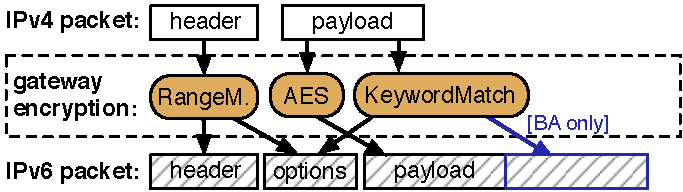
\includegraphics[width=3.0in]{fig/packet.pdf}
\caption{Packet encryption at the gateway. Patterned squares indicate encrypted data. Only for BA  middleboxes,  KeywordMatch produces additional encrypted data.  \label{fig:packet}}
\end{figure}





\begin{figure*}[t!]
\centering
  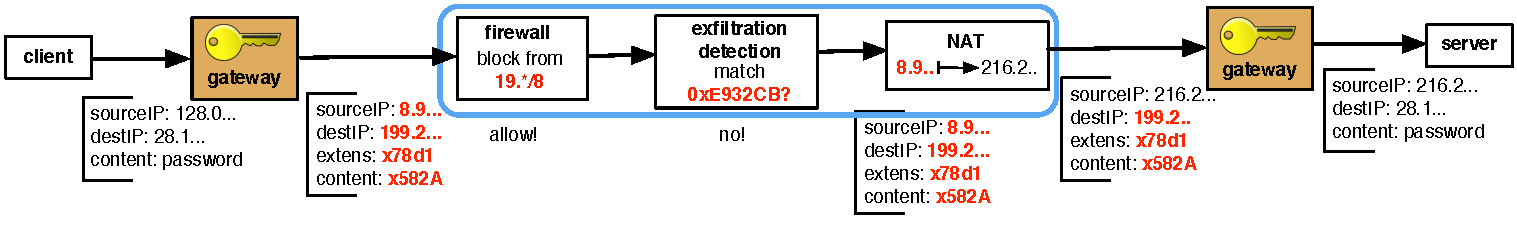
\includegraphics[width=6.7in]{fig/packetpath.pdf}
\caption{Example of packet flow through a few middleboxes. Red in bold indicates encrypted data. \label{fig:packetflow}}
\end{figure*}



To protect privacy of the traffic, \sys encrypts all the traffic passing through the service provider (SP).
\sys encrypts IP addresses, ports, and the payload of the packet, thus protecting the privacy of all these parameters. 
As in Fig.~\ref{fig:sys-overview}, the gateway has a secret key $k$; in the setup with two gateways, they share
the same secret key. The gateway encrypts all traffic going to the service provider using \sys's encryption schemes.
The middleboxes at SP process {\em encrypted traffic} using \sys's protocols. 
After the processing, the middleboxes
will produce encrypted traffic which SP sends back to the gateway. The gateway decrypts the traffic using the key $k$.

Throughout this process, middleboxes at SP handle only encrypted traffic and never get the decryption key. This ensures
that an attacker that steals all the data from SP will  see only encrypted traffic, which protects the privacy of the 
traffic. 



\mypara{Two types of middleboxes} \sys enables encrypted operation for {\em all} typical middleboxes in outsourcing scenarios, despite substantial differences in how the middleboxes operate, what packet data they access, and whether they modify or merely observe packets.
  We classify middleboxes in  two broad categories based on the type of encrypted fields  they compute on.

\noindent{\it Header-Only Middleboxes:} operate over packet headers (\eg{}, IP, TCP, or even HTTP headers) on a packet-by-packet basis.
Examples  include IP Firewalls and Network Address Translators (NATs). 

\noindent{\it Bytestream-Aware Middleboxes:} these middleboxes operate over a TCP bytestream -- the concatenation of all {\it payloads} -- and hence must keep copies of the data transmitted for each connection.
  For example, many Intrusion Detection Systems (IDS) are bytestream-aware; in order to detect attack signatures that span across multiple packets they keep a buffer  with copies of each payload it has forwarded.
  %It uses these payloads to reconstruct the TCP bytestream, just as the client will observe at the application layer; the IDS can then scan this bytestream for malicious substrings.
%%Because of this reconstruction cost, and the complexity of the computation over the reconstructed data, 
Most bytstream aware middleboxes achieve lower throughput than header-only middleboxes.

 Web proxies are a special case: even though this middlebox reconstructs the bytestream, the only computation on encrypted data is on the HTTP header, so we classify them as a HO middlebox. 
 
 
  
%  Web proxies are also bytestream-aware; rather than keeping a copy of packets the proxy forwards, the proxy performs {\it session termination}. 
%  When a client opens a new HTTP connection, a typical proxy will capture the client's SYN packet and open a new connection to the client, as if it were the web server the client wished to connect to. 
%  The proxy also maintains second connection in the background to the original web server, as if it were the client. 
%  Session termination allows the proxy to cache entire images (which usually span multiple packets) and respond to client requests with cached data as if it were the server.
 
 
 %For these applications, the gateway in \sys maintains no per-connection state, and its computation is very lightweight.  
 %For these middleboxes, the gateway in \sys maintains some state per connections, namely it reconstructs the TCP bytestream. 

 
 
  In Table~\ref{tab:apps-ops}, we list the type of each  middlebox in \sys. 
  
  %As we will see, to support header-only middleboxes, the \sys gateway can also operate in a header-only fashion, encrypting each header field (\eg{}, IP address, port number) independently.
  %However, to support bytestream-aware appliances, the \sys gateway also needs to  be bytestream aware, in order to encrypt the concatenation of packet payloads.
 % The one exception to this rule -- that header-only middleboxes can be served by a header-only gateway, while bytestream-aware middleboxes require a bytestream-aware gateway -- is web proxying.
%  Proxies are bytestream-aware, but can be served by a header-only middlebox when they do not allow pipelined requests.
  %As we will discuss in \S\ref{sec:proxies}, the gateway can encrypt the HTTP header values on a packet-by-backet basis without requiring any TCP bytestream reconstruction so long as HTTP pipelining is not enabled. 


\mypara{Packet encryption}
%Middleboxes at the cloud operate over the encrypted values in each packet, and do not have access to the decrypted data.
The gateway always generates IPv6 packets as output to the cloud, regardless of whether the input packets from the enterprise are v4 or v6. The tunnel connecting the gateway to the cloud may be either v4 or v6.
As we will see in the following section, our RangeMatch scheme requires 128 bits to encode encrypted IP addresses.
i% addresses. Nevertheless, this is not unusual considering that more and more enterprises are switching to IPv6. Moreover, \sys does not require the client and the server to use IPv6: they can use IPv4 in which case the gateway converts the packet to IPv6 using the Stateless IP/ICMP Translation Algorithm (SIIT)~\cite{SIIT}.

Fig.~\ref{fig:packet} shows how the gateway encrypts each packet.
All IP addresses and ports in the header are encrypted with RangeMatch.
As we will see, all header-based middleboxes can operate directly on RangeMatch encrypted values as if they were normal IP addresses and port values.
However, RangeMatch is not reversible: it is not possible to go from ciphertext back to plaintext. Hence, we also place normal AES \clan{(Do we say AES or stream cipher?)} encrypted values for the encrypted header fields in the IPv6 options header; these values are ignored by the middleboxes but used only at the gateway to decrypt packets after they return from the cloud.
Some network appliances are commonly configured to drop packets with IP options; these middleboxes must be configured under \sys to permit packets with \sys options to pass through.
Finally, bytestream-aware middleboxes which operate on the packet payload do not operate directly on the payload: we modify these middleboxes to read KeywordMatch values for the payload from either the options header or a secondary metadata channel which travels alongside the normal packets.
The payload itself is encrypted with standard AES, but not operated on by any middlebox.
\todo{RALUCA PLEASE READ: Kay found this section confusing so I tried to clarify. Can you make sure this is correct/makes sense?}

\mypara{Packet flow example}
To understand \sys, Fig.~\ref{fig:packetflow} shows the end-to-end flow of a packet through three example middleboxes in the cloud.  First,  the gateway encrypts the packet as explained above. The packet passes through the firewall which tries to match the encrypted information from the header against its encrypted rule, and decides to allow the packet. Next, the exfiltration device checks for any suspicious (encrypted) strings on the extension of the packet's payload, and not finding any, it allows the packet  to continue to the NAT. The NAT maps the source IP address to a different IP address. Back at the gateway, the gateway decrypts the packet. 

On top of \sys's encryption, the gateway can use SSL  to secure the communication to SP.  It can use SSL also on the links client-G and G-server.


